\documentclass{article}
\usepackage{amsmath}
\usepackage{multicol}
\usepackage{blindtext}
\usepackage{geometry}
\usepackage{makecell}
\usepackage{setspace}
\usepackage{graphicx}
\usepackage{float} 
\usepackage{subfigure}
 \geometry{
 a4paper,
 left=5mm,
 top=3mm,
 right=2mm,
 bottom=3mm,
 }
 \usepackage[fontsize=8pt]{fontsize}
 \linespread{1.0}
\begin{document}
\thispagestyle{empty}
\setstretch{1.0} 
\begin{multicols}{3}

  \noindent\textbf{Harmonic Motion}\\
  $A \sin(\omega t + \phi)$\\
  $A \exp^{i(\omega t + \phi)} = A(\cos(\omega t + \phi) + i\sin(\omega t + \phi))$\\
  \begin{equation*}
    m\ddot{x}+c\dot{x}+km=0
  \end{equation*}
\begin{equation*}
  \ddot{x}+\frac{c}{m}\dot{x}=\frac{k}{m}x=0
\end{equation*}
\begin{equation*}
  \ddot{x}+2\xi\omega_{n}\dot{x}+\omega^{2}x=0
\end{equation*}
$\omega_{n}$ is the natural frequency for undamped system.

  \underline{critical damping} $C_{c}=2\sqrt{kM}$\\
  \underline{Damping ratio} $\xi =\frac{c}{2m\omega_{n}}$\\
  \underline{Natural Frequency} $\omega_{n}=\sqrt{\frac{K}{M}}$\\
  \underline{Damped natural frequency} $\omega_{d}=\sqrt{1-\xi^{2}}\omega_{n}$\\
  \underline{EOM of Damped System}\\
  $x=e^{-\varsigma \omega_{n}t} (\frac{\dot{x}_{0}+\varsigma \omega_{n}x_{0}}{\omega_{d}}\text{sin}\omega_{d}t+x_{0}\text{cos}\omega_{d}t)$\\
  $\omega=2\pi f=2\pi N/60$, N:rpm

\noindent\textbf{Mearsure damping}\\
1.decay method using free respound (time domain):
excite the structure(impact or perturbation), mearsure response,plot decay curve.
\begin{equation*}
  \delta=\frac{1}{n}\text{ln}\frac{x_{i}}{x_{i+n}}, \xi =\frac{\delta}{2\pi}
\end{equation*}
2.Half-power method(frequency domain): need a shaker with a force transducer to excite the structure. Use a Random excitation and mearsure the response-force transfer function. Locate the peak position in the spectrum.
Sweep the resonance area using hamonic excitations.
\begin{equation*}
  G=20\text{log}A,20\text{log}\sqrt{2}=3\text{dB}
\end{equation*}

Find the frequencies giving $X_{max}/\sqrt{2}$ (-3dB),$\xi =\frac{\Delta \omega}{2\omega_n}$

\noindent\textbf{Free Vibration Response}\\
\begin{equation*}
  {x}=\sum_{r=1}^{2}A_{r}u_{r}\text{sin}(\omega_{r}t+\phi^{r})
\end{equation*}
where $A_{r}$ is modal contribution factor, $u_{r}$ is modal shape

\noindent\textbf{general method of EOM}\\
Newtonian approach,Energy approach, variational approach,
method of infuluence of coefficient$[k]$

for static system:$\ddot{q}=\dot{q}=0$
\begin{equation*}
  [q]=[a_{ij}][F]=[k]^{-1}[f]
\end{equation*}
where $a_{ij}$ is the displacement at $i$ due to a unit force applied at $j$.
$k_{ij}$ is the force required at $i$ for keeping the system static equlibrium when a unit displacement is imposed at $j$.

\noindent\textbf{Isolation}\\
\underline{Transmitted} $F_{t}=\sqrt{|kx|^{2}+|C\dot{x}|^{2}}$ (amplitude with $90^{o}$ phase)
\begin{equation*}
  TR=\frac{\sqrt{1+(2\xi r)^{2}}}{\sqrt{(1-r^{2})^{2}+(2\xi r)^{2}}}, r=\frac{\omega}{\omega_{n}}
\end{equation*}
$TR<1$ only for $r> \sqrt{2}$.\\
$\omega_{n}=\sqrt{K/M}=\sqrt{\frac{g}{\delta}}$, $\delta$ is static deflection. \\
$\xi= \frac{C}{C_{c}}=\frac{C}{2\sqrt{KM}}$, $\xi \downarrow, TR \downarrow$

\noindent\textbf{Second Order Differential Equation}\\
 When $b^2 - 4ac > 0$, two different roots $r_1, r_2$, $y = C_1\exp^{r_1 x} + C_2\exp^{r_2 x}$ \\
 When $b^2 - 4ac = 0$, two equal roots $r$, $y = C_1 e^{r x} + C_2 x e^{r x}$\\
 When $b^2 - 4ac < 0$, two equal roots $a \pm bi$, $y = e^{ax} [C_1 \cos(b x) + C_2 \sin(b x)]$

\noindent\textbf{Forced Vibration}\\
\underline{Harmonic force} $F\sin\omega t$, $m\ddot{x} + c\dot{x} + kx = F\sin\omega t$
\begin{equation*}
  x(t)=\frac{F/k}{\sqrt{(1-r^{2})^{2}+(2\xi r)^{2}}}\text{sin}(\omega t-\phi)
\end{equation*}
$\phi=\text{arctan}(\frac{2 \xi \omega_{n}\omega}{\omega_{n}^{2}-\omega^{2}})=\frac{2\xi r}{1-r^{2}}$\\
\underline{Impulsive response} $x=h(t) = \frac{1}{M\omega_n}\sin(\omega_n t)$\\
\underline{Transient response}  $x = \int_0^t F(\xi) h(t-\xi) d\xi$\\
\underline{Transient response with damping}\\
$h(t)=\frac{e^{-\varsigma}\omega_{n}t}{M\omega_{n}\sqrt{1-\varsigma^{2}}}\text{sin}\omega_{n}\sqrt{1-\varsigma^{2}}t$

\noindent\textbf{Virtual Work}\\
The virtual work of a static system is always 0.\\
\underline{D'Alembert's Principle}
\begin{equation*}
  \sum_k (F_k - m \ddot{r_k}) \delta r_k = 0
\end{equation*}

\noindent\textbf{Decoupling}\\
1. \underline{Solve eigenvalue Pb}
$[[k]-\omega^{2}[M]][u]=0$
get $\omega_{r}^{2},[u_{r}]$.\\
2. \underline{Transformation of coordinate}\\
$[q(t)]=[[u_{1}],[u_{2}],...][\eta(t)]$\\
3. \underline{Decoupling}\\
$[u]^{T}[M][u][\ddot{\eta(t)}]+[u]^{T}[K][u][\eta(t)]=[u]^{T}[Q]$\\
4. \underline{Transformation of IC} $[\eta(0)]=[u]^{-1}[q(0)]$
 $$
 \frac{1}{\omega_{r}}\int_{0}^{t}N(\zeta)\text{sin}\omega_{r}(t-\zeta)d\zeta+\eta_{r}(0)\text{cos}\omega_{r}t+\dot{\eta}_{r}(0)\frac{\text{sin}\omega_{r}t}{\omega_{r}}
 $$
5. \underline{Original q} $[q(t)]=[u][\eta(t)]$\\
\underline{Remark}:$\{[M]^{-1}[K]\}[\bar{x}]=\omega^{2}[\bar{x}]$

\noindent\textbf{Quantities}\\
\underline{Torque} $\tau = Fr \sin\theta$\\
\underline{Rotational Inertia} $I=\frac{1}{2}mr^2$ (For rigid)\\
\underline{Rotational Torque} $\tau = I\alpha$, $\alpha = \dot{\omega}$\\
\underline{Rotational Kinetic} Energy $E_{rotational}=\frac{1}{2}I\omega^2$\\

\noindent\textbf{Lagrange Equation}
\begin{equation*}
  \frac{d}{dt}\frac{dT}{d\dot{q_i}} - \frac{dT}{dq_i} + \frac{dU}{dq_i} = 0
\end{equation*}
Let $L = T - U$,
\begin{equation*}
  \frac{d}{dt}\frac{dL}{d\dot{q_i}} - \frac{dL}{dq_i} = 0
\end{equation*}

\noindent\textbf{Theory of Elasticity}\\
\underline{Stress $\sigma$} distribution of internal force within a body $\frac{F}{A}$\\
\underline{Stain $\varepsilon$} deformation within a body $\frac{\Delta L}{L}$\\
\underline{Young's Modulus $E$} In elastic region, $\sigma = E\varepsilon$\\
\underline{Shear Force $\tau$} conduct by transverse force $\frac{F}{A}$\\
\underline{Hook's law}
  \begin{equation*}
    \sigma=\frac{N}{s}=E\varepsilon=E\frac{\partial u}{\partial x}
  \end{equation*}
\underline{Deformation-Displacement relationship}\\
  $\varsigma=\frac{1}{2}(\frac{\partial u_{i}}{\partial x_{j}}+\frac{\partial u_{j}}{\partial x_{i}})$\\

\underline{Deformation-Displacement relationship}\\
  $\epsilon = \frac{1}{2}(\frac{\partial u_{i}}{\partial x_{j}}+\frac{\partial u_{j}}{\partial x_{i}})$\\

  \noindent\textbf{Flexural beam}\\
  \underline{Displacement} $w$\\
  \underline{Rotation} $\frac{\partial w}{\partial x}$\\
  \underline{Moment} $M=EI\frac{\partial^{2} w}{\partial x^{2}}$\\
  \underline{Shear Force} $\frac{\partial M}{\partial x}=\frac{\partial }{\partial x}(EI \frac{\partial^{2}w}{\partial x^{2}})$

  \noindent\textbf{Rayleigh method}\\
  Since $T_{max} = U_{max}$, assume $w(x,t) = y(x) \sin\omega t$,
      \begin{equation*}
        \omega^2 =\frac{U_{max}}{T_{max}}=\frac{\int_0^l EI(\frac{d^2y}{dx^2})^2 dx}{\int_0^l \rho s y^2 dx}
      \end{equation*}
  This method is more accurate if assumed function $y(x,t)$ \textbf{satisfy} all BCs. not only geometrocal BC.

  General, $y(x)\neq y_{s}(x)$,  $y(x)=\sum_{i=1}^{\infty}c_{i}y_{i}(x)$(modal superposition).
  
  Therefore, $\omega^{2}=\omega^{2}_{r}+\sum_{i=1\neq r}(\frac{c_{i}}{c_{r}})^{2}\omega_{i}^{2}$. So $\omega>\omega_{r}$.
  
  \noindent\textbf{Ritg method}\\
  1. Decompose $w(x,t) = a_0(t) + a_1(t)x + a_2(t)x^2$\\
  2. Use BC to simplied $w(x,t)$ \\
  3. Calculate $T$ and $U$\\
  4. Solve Lagrange $L = T - U$, get $\omega$ and mode shape

  \noindent\textbf{Math}\\
  \underline{Inverse Matrix of 2 dims}
  \begin{equation*}
    \begin{bmatrix}
      a & b \\
      c & d
    \end{bmatrix}^{-1} =
    \begin{bmatrix}
      d & -b \\
      -c & a
    \end{bmatrix}
  \end{equation*}
  $\cos\theta = \frac{a^2+b^2-c^2}{2ab}$\\

  \noindent\textbf{Hamilton function}
  \begin{equation*}
    H=\int_{t_{1}}^{t_{2}}(T-V+W_{F})\text{d}t
    =\int_{t_{1}}^{t_{2}}\int_{0}^{L}F(u,u_{,t},u_{,x})\text{d}x\text{d}t
  \end{equation*}

  \noindent\textbf{Eular equation}
  \begin{equation*}
    \frac{\partial F}{\partial u}-\frac{\partial}{\partial x}(\frac{\partial F}{\partial u_{,x}})-\frac{\partial}{\partial t}(\frac{\partial F}{\partial u_{,t}})=0
  \end{equation*}

  \noindent\textbf{Last chapter}\\
  \underline{peak-peak}: the level of a vibration signal
  \underline{average}: $\frac{1}{T}\int_{0}^{T}|x|\text{d}t$, $T$ is acquisition time.
  \underline{RMS(root mean Square)}: $\sqrt{\frac{1}{T}\int_{0}^{T}x^{2}(t)\text{d}t}$,related  to the energy.
  \underline{Parameter} to measure: Low frequency $\rightarrow$ Displacement; High frequency $\rightarrow$ Acceleration.

\noindent\textbf{Piezoelectric Accelermoeters}\\
\underline{EOM} $m \ddot{x} = -c(\dot{x}-\dot{y}) - k(x-y)$
\begin{equation*}
  m\ddot{z}+c\dot{z}+kz=m\ddot{y}
\end{equation*}
  \underline{Deformation of Spring}: $Z = \frac{1}{\omega_n^2} \frac{\omega^2Y}{\sqrt{(1-r^2)^2+(2\xi r)^2}} = A Y$
  \underline{Seismometer}: Low natural frequency $r\rightarrow\infty$, $Z = Y$. With $\xi=0.7$, the actual application range begins from $2.5\omega_n$. (Seismic frequency begins from $2.5\omega_n$)\\
  $A=\frac{r^{2}}{\sqrt{(1-r^{2})^{2}+(2\xi r)^{2}}}\rightarrow 1$\\
  \underline{Accelerometers}: High natural frequency $r\rightarrow0$, $Z = \omega^2Y$. Application range is below $0.2\omega_n$. $\xi$ always sets to $0.7$ for a wider range and a minimum phase distortion.\\
  $B=\frac{1}{\sqrt{(1-r^{2})^{2}+(2\xi r)^{2}}}$\\
\underline{practical design of Accelerometers}\\
1.the bigger the Accelerometer, the higher its sensitivity, the smaller is its useful frequency range.\\
2. samll accelerartion are often used to mearsure high level vibrations.\\
3. transverse sensitivity should be less than $4\%$.\\
4. When testing light structure, small accelerometer should be used to avoid possible interferences.\\
\underline{calibration} back-to-back,using a calibration exciter.\\
\underline{mounting accelerartion}: Stud and wax (restriced to $40^{o}$) is better.\\
\underline{amplifier}:voltage amplifier(change with cable length), charge amplifier.\\
The majority of preamplifiers used today are charge amplifiers as they are not affected by cable length or resistance changes within reasonable limits.\\

\noindent\textbf{Excitation}\\
\underline{Electromagnetic Shaker}\\
  1. Harmonic excitation:at fixed frequency sweeping.
  2. Random excitation: white noise with  a flat continuous spectrum in Frequency domain
\underline{Hammer} impact excitation

\noindent\textbf{Experimental modal analysis}\\
Determine the natural frequency, modal damping, mode shape.\\
Frequency response fuction(FRF) measurement applied to lightly damp and signal-degree-of-freedom.\\
\underline{modal test on simple structures}
1.Use a shaker with a force transducer or a hammer to excite the structures.\\
2.Use a random excitation or impact to excite the structure and measure the FRF curve.\\
3.Locate the peak position in the spectrum to estimate the natural frequencies.\\
4.use a sweeping sine excitation to measure each resonance peak.\\
5.Use the half-power (or –3dB) method to measure damping.At resonance, measuring the displacement at different points gives the natural mode shape of the structure.\\

  \noindent\textbf{Quiz}\\
  \underline{Differences between Bernoulli and Timoshenko} Bernoulli beam ingnores shear deformation and rotation energy. Timoshenko beam need to be used while beam is short or has large soft deformation, like sandwich composite beams.\\
  \underline{why heavy inertial mass for vibration?} $\omega_n=\sqrt{k/m}$ and $r=\omega/\omega_n$\\
  \underline{Criterion for selecting isolator} $k \downarrow, c \downarrow$ \\
  \underline{Vibration Reduction}\\
  1. Adding an additional constraint (e.g. local support or stiffness) to the place with maximum displacement of the panel.\\
  2. Increasing structural damping by adding a small piece of viscoelastic coating on the place with maximum deformation of the panel. \\
  3. Add inertial mass to motor.\\
  \underline{TODO} The natural frequency gets smaller when the effct of shear deformation and rotational inertia are consideres. Add stiffness.\\
  \underline{Rayleigh overestimates natural frequency} \\
  $\omega^2 = \omega_r + \sum_{i\neq r}(\frac{C_i}{C_r}\omega_i)$, the result is contributed by other modals. Thus the real natural frequency $\omega_r$ is always lower than Rayleigh result $\omega$.\\
  \underline{Effect of shear deformation and rotational inertia} \\
  1. Effect of rotation $<$ Effect of shear \\
  2. $\omega_n < \omega_n(Bernoulli)$\\

  \noindent\textbf{Assignment}\\
  1. critical damping $\xi=1$, the system return to its equlibrium position within the shortest time without vibration.
  $\xi>0$: over-Damped:no Vibration.\\
  2. torsion $\tau=\frac{\text{d}L}{\text{d}t}=I\alpha$, $L=I\omega$.\\
  3. critical speed is natural frequency. damping factor(coefficient) is damping ratio.\\
  4. spring with mass: $v(x)=\frac{y}{l}\dot{x}$.
  \begin{equation*}
    T_{spring}=\int_{0}^{l}\frac{1}{2}\frac{M}{l}(\frac{y}{l}\dot{x})^{2}\text{d}y
    =\frac{1}{6}M\dot{x}^{2}
  \end{equation*}
  5. $T_{disk}=\frac{1}{2}J\dot{\theta}^{2}$,$J=\frac{1}{2}Mr^{2}$.
 \end{multicols}

  \begin{table*}[htbp]
  % \begin{table}[H]
    \centering
    \caption{comparison}
    \begin{tabular}{|c|c|c|c|c|}
      \hline
      Name&string&Longitudinal beam& Flexural beam&plate\\
      \hline
      T
      &$\frac{1}{2}\int_{0}^{l}m(x)(\frac{\partial y}{\partial t})^{2}\text{d}x$
      &$\frac{1}{2}\int_{0}^{l}\rho s(\frac{\partial u}{\partial t})^{2}\text{d}x$
      &$\frac{1}{2}\int_{0}^{l}\rho s(\frac{\partial u}{\partial t})^{2}\text{d}x$
      &$\frac{1}{2}\int_{0}^{l_{1}}\int_{0}^{l_{2}}\rho h(\frac{\partial w}{\partial t})^{2}\text{d}x_{1}\text{d}x_{2}$\\
      \hline
      V&$\frac{1}{2}\int_{0}^{l}T(\frac{\partial y}{\partial x})^{2}\text{d}x$
      &$\frac{1}{2}\int_{0}^{l}Es(\frac{\partial^{2} w}{\partial x^{2}})^{2}\text{d}x$
      &$\frac{1}{2}\int_{0}^{l}EI(\frac{\partial^{2} w}{\partial x^{2}})^{2}\text{d}x$
      &$\frac{1}{2}\int_{v}\sigma_{ij}\varepsilon_{ij} \text{d}$v\\
      \hline
      \makecell[c]{Motion \\Equation}&$T\frac{\partial ^{2}y(x,t)}{\partial x^{2}}=m(x)\frac{\partial^{2}y(x,t)}{\partial t^{2}}$
      &$\frac{\partial^{2}u(x,t)}{\partial x^{2}}-\frac{\rho}{E}\frac{\partial^{2}u}{\partial t^{2}}=0$
      &\makecell[c]{$\frac{\partial ^{2}}{\partial x^{2}}(EI\frac{\partial^{2}w}{\partial x^{2}})+\rho s \frac{\partial^{2}w}{\partial t^{2}}=$ \\ $-f(x,t)-\frac{\partial m(x,t)}{\partial x}$}
      &\makecell[c]{$D \bigtriangledown ^{4}w+\rho h \frac{\partial ^{2}}{\partial t^{2}}=f$\\
      $D=\frac{Eh^{3}}{12(1-v^{2})}$\\$\bigtriangledown^{4}=\frac{\partial ^{4}}{\partial x_{1}^{4}}+2\frac{\partial ^{4}}{\partial x_{1}^{2}\partial x_{2}^{2}}+\frac{\partial ^{4}}{\partial x_{2}^{4}}$}\\
      \hline
      \makecell[c]{boundry\\ condition}&fixed $y(0,t)=0$&\multicolumn{3}{|c|}{\makecell[c]{
        Simply-Supported $w \mid_{0 \text{ and } l} = 0$, $\frac{\partial^2 w}{\partial x^2} \mid_{0 \text{ and } l} = 0$\\
        Clamped-Clamped $w \mid_{0 \text{ and } l} = 0$, $\frac{\partial w}{\partial x} \mid_{0 \text{ and } l} = 0$\\
        Free-Free $\frac{\partial^2 w}{\partial x^2} \mid_{0 \text{ and } l} = 0$
        }}\\
      \hline
      \makecell[c]{normal\\ mode}& \makecell[c]{$\omega=\frac{n\pi}{l}\sqrt{\frac{T}{m}}$ \\$Y=A \text{sin}(\frac{n\pi}{l}x)$}
      &\makecell[c]{$\omega=\frac{n\pi}{l}\sqrt{\frac{E}{\rho}}$\\ $u=A \text{sin}(\frac{n\pi}{l}x)$}
      &\makecell[c]{
        $\omega=\frac{n^{2}\pi^{2}}{L^{2}}\sqrt{\frac{EI}{\rho s}}$
        $y=\text{sin}(\frac{n \pi}{L}x)$\\
        general $y=a\text{cos}\alpha x+b\text{sin}\alpha x$\\
        $+c \text{cosh}\alpha x+d \text{sinh}\alpha x$\\
        $\alpha^4 = \frac{\rho S \omega^2}{EI}$
      }
      &\makecell[c]{
        $w(x,y,t)=W(x,y)e^{i\omega t}$\\
        Simply-supported plate:\\
        $\omega=\sqrt{\frac{D}{\rho h}}[(\frac{m\pi}{a})^{2}+(\frac{n \pi}{b})^{2}]$\\
      $W=A\text{sin}\frac{m\pi x}{a}\text{sin}\frac{n \pi y}{b}$\\
      \textbf{$\rho$ is volume density and $\rho h$ is area density}
      }\\
      \hline
    \end{tabular}
  \end{table*}


\begin{table*}[htbp]
% \begin{table}[H]
    \centering
    \caption{Displacement Filed}
    \begin{tabular}{c|l}
    \hline
      General Beam &
      \makecell[l]{
      $u_{1}(x_{1},x_{2},x_{3},t)=u_{1}^{0}(x_{1},0,0,t)+x_{2}u_{1}^{2}(x_{1},0,0,t)+x_{3}u_{1}^{3}(x_{1},0,0,t)$\\
      $u_{2}(x_{1},x_{2},x_{3},t)=u_{2}^{0}(x_{2},0,0,t)+x_{2}u_{2}^{2}(x_{1},0,0,t)+x_{3}u_{2}^{3}(x_{1},0,0,t)$\\
      $u_{3}(x_{1},x_{2},x_{3},t)=u_{3}^{0}(x_{3},0,0,t)+x_{2}u_{3}^{2}(x_{1},0,0,t)+x_{3}u_{3}^{3}(x_{1},0,0,t)$\\
      $x_{2}u_1^2, x_{3}u_1^3$ Rotation \\
      $x_{2}u_3^2, x_{3}u_2^3$ Torsion \\
      $x_{2}u_2^2, x_{3}u_3^3$ Poisson \\
      } \\
      \hline
      Logituditnal Beam &
      \makecell[l]{
      $u_{1}(x_{1},x_{2},x_{3},t)=u_{1}^{0}(x_{1},0,0,t)$\\
      $u_{2}(x_{1},x_{2},x_{3},t)=0$\\
      $u_{3}(x_{1},x_{2},x_{3},t)=0$\\
      } \\
      \hline
      Flexural Beam &
      \makecell[l]{
      $u_{1}(x_{1},x_{2},x_{3},t)=x_{2}u_{1}^{2}(x_{1},t)$\\
      $u_{2}(x_{1},x_{2},x_{3},t)=u_{2}^{0}(x,t)$\\
      $u_{3}(x_{1},x_{2},x_{3},t)=0$\\
      for Bernoulli beam \\
      $u_{1}^{2}(x,t)=-\frac{\partial u_{2}^{0}}{\partial x}(x,t)$\\
      } \\
      \hline
      Plate &
      \makecell[l]{
      Timoshenko-Mindlin plates\\
      $u_{1}(x_{1},x_{2},x_{3},t)=x_{3}u_{1}^{3}(x_{1},x_{2},t)$\\
      $u_{2}(x_{1},x_{2},x_{3},t)=x_{3}u_{2}^{3}(x_{1},x_{2},t)$\\
      $u_{3}(x_{1},x_{2},x_{3},t)=u_{3}^{0}(x_{1},x_{2},t)$\\
      Love-Kirchoff plate\\
      $u_{1}=-x_{3}\frac{\partial w}{\partial x_{1}}$\\
      $u_{2}=-x_{3}\frac{\partial w}{\partial x_{2}}$\\
      $u_{3}=w$\\
      }\\
      \hline
    \end{tabular}
\end{table*}


\begin{figure*}[h]
  \centering
  \subfigure[forced vibration response]{
    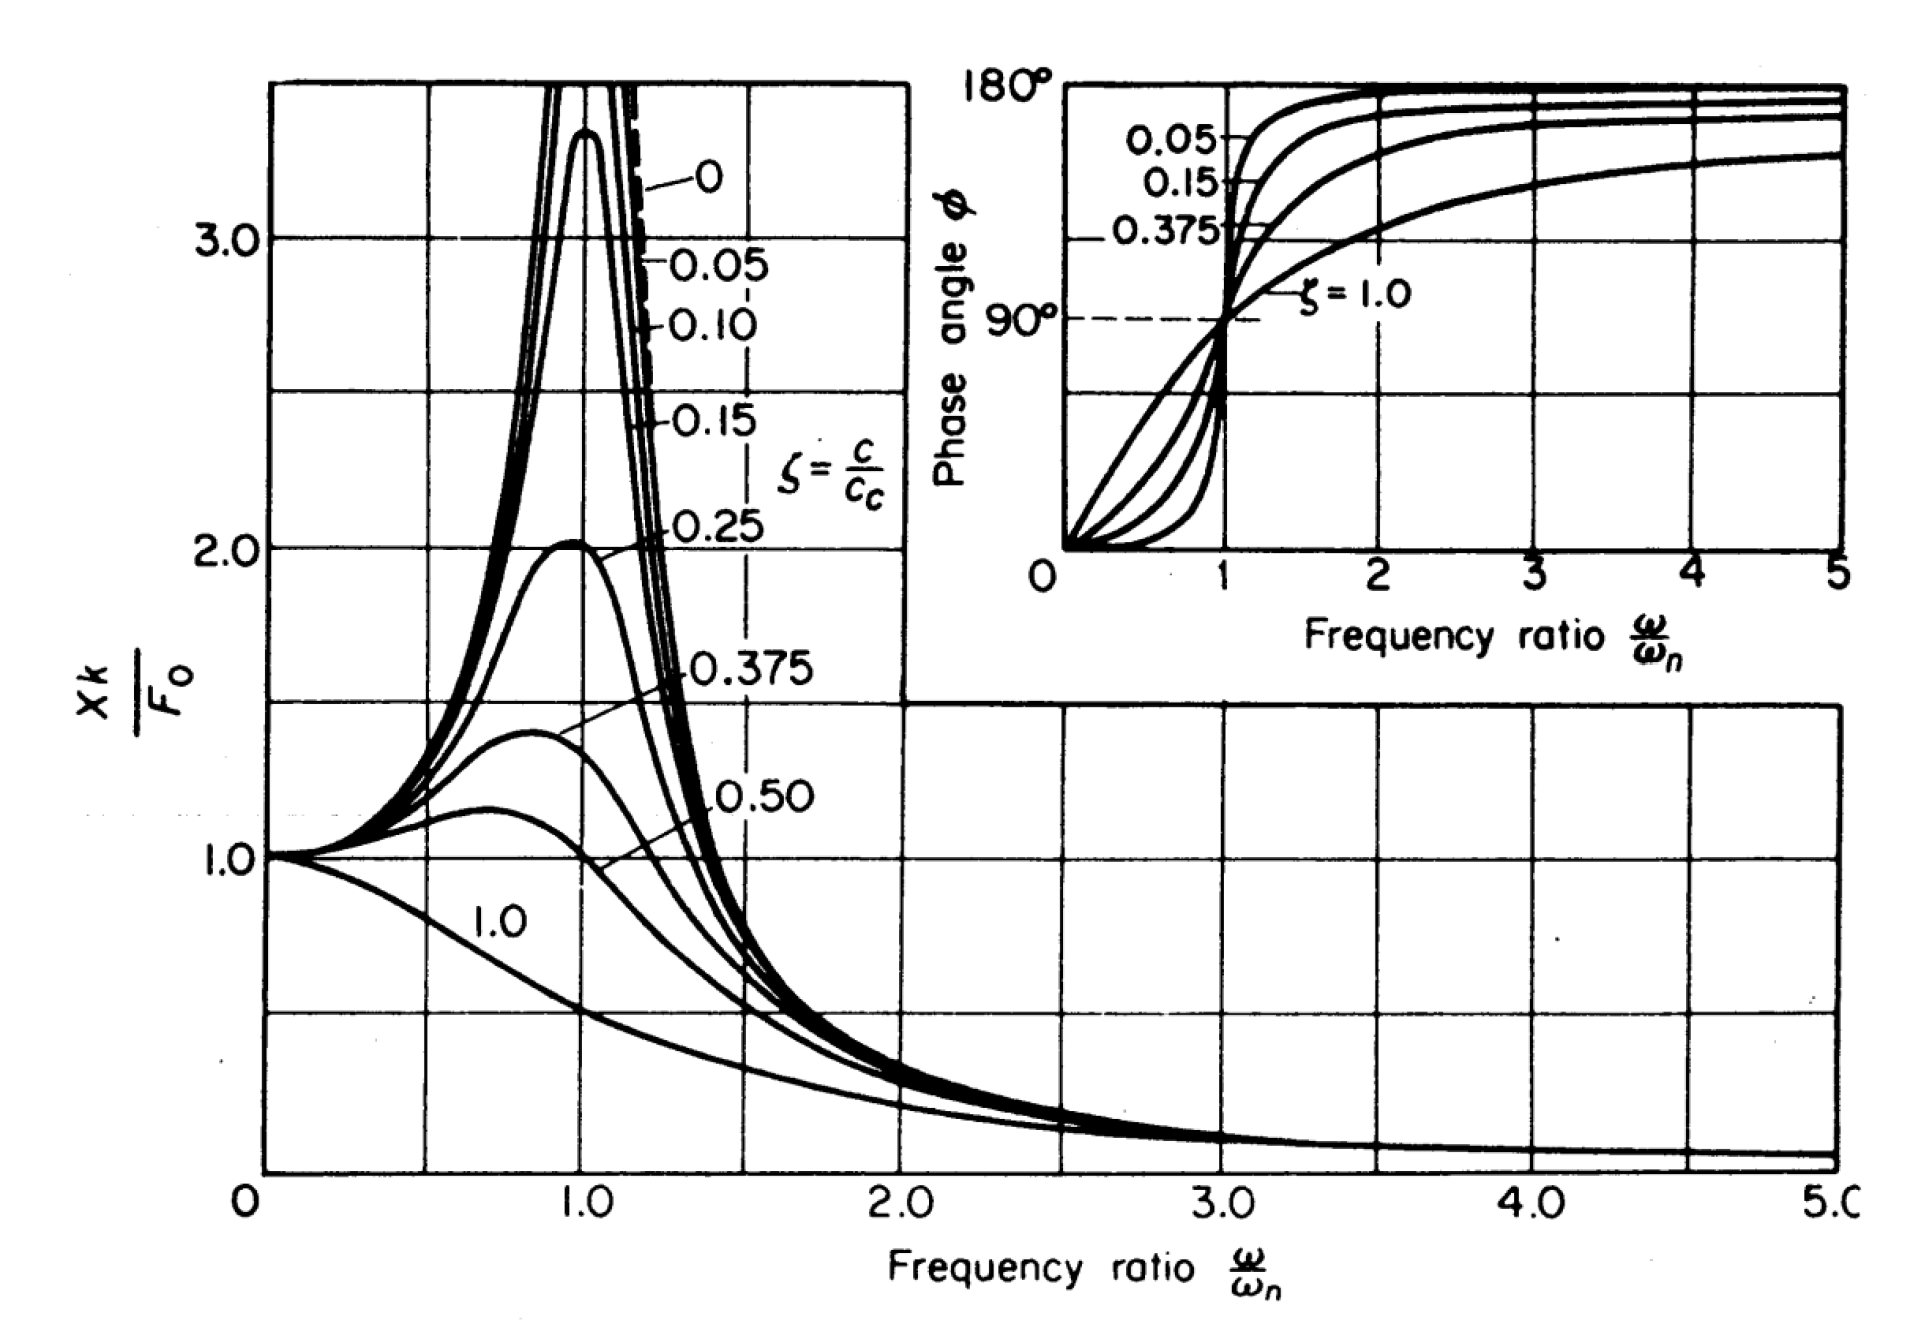
\includegraphics[width=0.27\textwidth]{Forced.png}
  }
 \subfigure[Isolator]{
  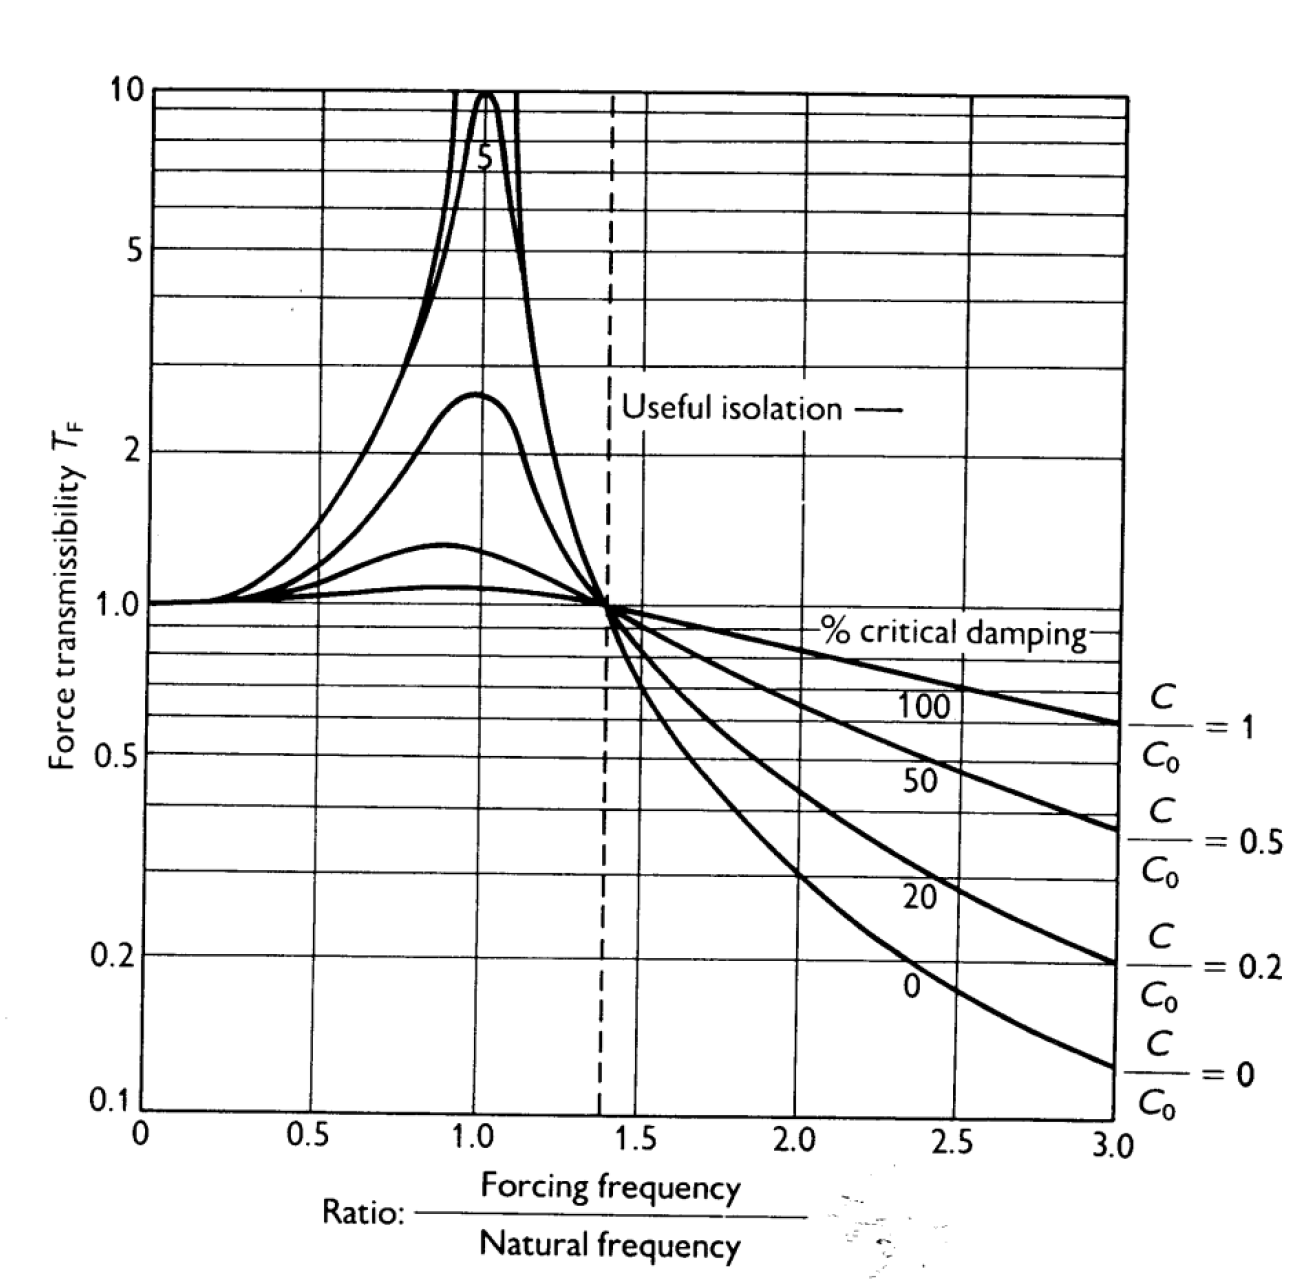
\includegraphics[width=0.27\textwidth]{Isolator.png}
 }
 \subfigure[excitation]{
  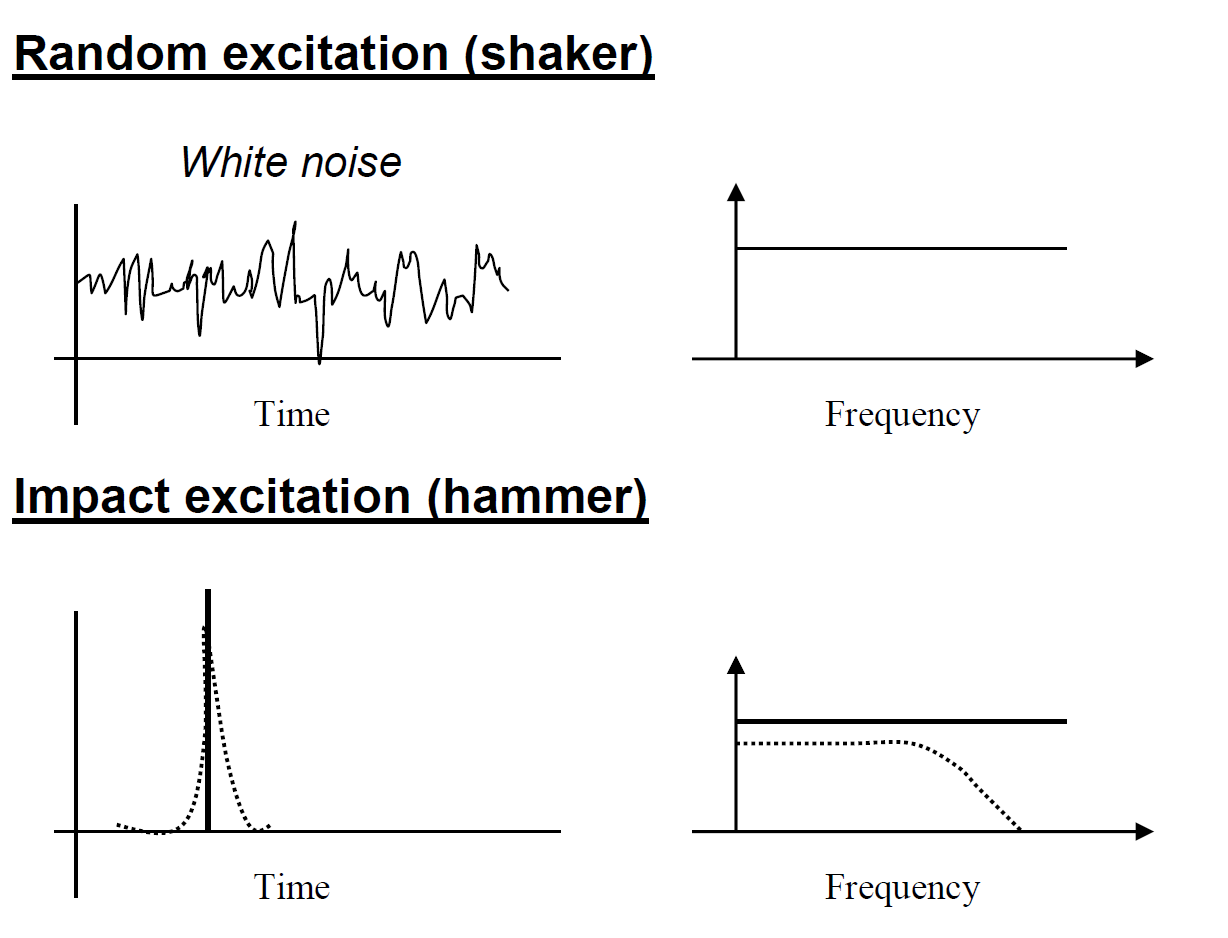
\includegraphics[width=0.27\textwidth]{excitation.png}
 }
\end{figure*}

\end{document}
